\documentclass[11pt]{article}
\usepackage[utf8]{inputenc}
\usepackage{amsmath,amssymb}
\usepackage{xcolor}
\usepackage{array}
\usepackage{natbib}
\usepackage{graphicx}
\DeclareGraphicsExtensions{.pdf,.png,.jpg}
\usepackage{float}
\usepackage[top=3cm, bottom=3cm, right=3cm, left=3cm]{geometry}
\usepackage{url}
\usepackage{booktabs}
\usepackage{enumitem}
% authblk not needed for blinded submission



% -------------------------------------------------------
% OUTLINE CONVENTIONS
%   \placeholder{text}  -- section not yet written
%   \todo{text}         -- decision or analysis still needed
% -------------------------------------------------------
\newcommand{\placeholder}[1]{\textcolor{gray}{\textit{[#1]}}}
\newcommand{\todo}[1]{\textcolor{red}{\textbf{[TODO: #1]}}}

\title{These Four First: A Robust Endogenous Baseline for Relational Event Sequences}

\author{Anonymous}

\begin{document}

\maketitle

% -------------------------------------------------------
\begin{abstract}
Which endogenous interaction mechanisms belong in a baseline relational event
model? We test for recurring endogenous patterns in 217 empirical interaction
sequences spanning ten social domains, evaluating a twelve-term candidate set
by forward AIC reduction. Four terms appear in the top-four
selection path in over 60\% of domains --- interaction-order constraints
(IOviolation, 94\%), prior sender initiation (SndInitiation, 88\%), rank-recency
of the most recent reverse-dyad event (RecRecencyRank, 65\%), and dyadic
repetition (Repetition, 61\%) --- with substantially diminishing returns at
step~4. Together they recover approximately 97\% of the maximum AIC improvement
achievable within this candidate set and represent three distinct behavioral
mechanisms: sequential ordering, dyadic persistence, and reverse-dyad recency.
Notably absent from this baseline are imitation (preferential attachment driven
by others' targeting behavior) and triadic closure terms, despite their
prominent roles in the network literature; both are absorbed by forward-dyad
history once SndInitiation and Repetition enter the model.
IOviolation's dominance as the most consistently selected term reflects the
near-universal importance of participation-shift norms across interaction
settings, even those that are not conversational. The step-2 composition
diverges ecologically: in high-visibility settings RecRecencyRank competes
closely with IOviolation at step~2 (38\% vs.\ 60\%), while in low-visibility
settings IOviolation dominates step~2 in 79\% of domains. These four terms are
not a sufficient model --- institutional context, status, demographic attributes,
and additional endogenous mechanisms all shape interaction --- but they are a
consistent baseline that researchers can include with confidence before
introducing substantive covariates. The cross-domain stability of this four-term
core --- spanning private messaging, classroom interaction, and gang violence ---
hints at a compact set of dyadic mechanisms that may constitute near-universal
building blocks of directed social interaction.
\end{abstract}

\noindent\textbf{Keywords:} relational event models; model selection; dyadic persistence;
reciprocity; sequential ordering; separable estimation; interaction mechanisms

\newpage

% -------------------------------------------------------
\section{Introduction}

Relational event models (REMs) offer a flexible framework for analyzing
the timing and sequencing of social interaction \citep{butts_sm_2008}.
REMs represent social interactions as conditioned on the full prior history of
interaction, allowing researchers to specify endogenous mechanisms ---
actors returning to established partners, reciprocating recent receipt,
conforming to turn-taking norms --- alongside exogenous covariates
capturing institutional context, demographic attributes, or other terms of interest. The
framework has been applied to email and phone communication, hospital
patient transfers, organizational deliberation, illegal market activity,
gang conflict, and more \citep{vu2017relational,kitts2017investigating,%
liang2014organizational,duxbury2021shining,gravel2023rivalries,%
renshaw2023modeling}, in each case producing substantively interpretable
estimates of theoretically motivated predictors.

A persistent challenge in applied REM research is model specification:
a substantial catalogue of endogenous mechanisms has been documented in
the literature \citep{butts2023relational}, but no consensus exists on
which subset any well-specified model must include. In practice,
researchers either include all available endogenous statistics --- risking
convergence issues, overfitting, and complicated interpretation --- or
select a subset on theoretical or disciplinary grounds, potentially omitting important endogenous terms.
Parsimonious models are generally preferable: they are more interpretable, more stable to fit, and
generalize more reliably in simulation and out-of-sample prediction.
But parsimony must be balanced against the risk of omission. An
endogenous mechanism left out of a model is often redistributed across the remaining predictors,
including exogenous covariates of substantive interest. A researcher
who omits a consistently important endogenous term risks attributing
real behavioral tendencies (e.g., actors returning to established partners,
following sequential rules) to institutional, demographic, or
organizational variables correlated with interaction history.

Here, we ask which endogenous terms are \emph{consistently first-selected}
across diverse empirical settings: the ones a researcher can include with
confidence that they contribute meaningfully regardless of domain. Prior
work has asked which terms are statistically significant within specific domains, and no general guidance on starting points currently exist to our knowledge. We address this gap by applying greedy
forward model selection to 217 empirical interaction sequences spanning
ten social domains, evaluating a twelve-term candidate set of endogenous
statistics and identifying where marginal AIC gains systematically plateau.
Because greedy selection is path-dependent, we corroborate the results with
two path-independent checks: univariate AIC rank at step~1 (which term fits
best with nothing else in the model) and leave-one-out AIC from the full
twelve-term joint model (which terms are most costly to remove). The same
four terms are identified by all three criteria.
The domains are deliberately diverse --- email and phone communication,
private messaging, face-to-face glances, gang violence, and international
conflict --- so that any term appearing consistently in the first four
selection steps across all of them is unlikely to be a domain-specific
artifact.

We find that four terms constitute the robust endogenous baseline: within
this twelve-term candidate set,
\textbf{SndInitiation} (whether $i$ has ever
previously sent to $j$), \textbf{IOviolation} (an indicator of participation-shift violations
in sequential ordering), \textbf{Repetition} (sender $i$'s
normalized prior send-share to receiver $j$), and \textbf{RecRecencyRank} (rank-based recency of
the most recent $j \to i$ event) each appear in the top-four
selection path in over 55\% of domains when frequencies are computed as
domain-weighted averages (SndInitiation: 94\%, IOviolation: 91\%,
Repetition: 61\%, RecRecencyRank: 55\%). Domain weighting is essential
because two domains --- Gang Violence ($n=100$) and Glances ($n=62$) ---
together account for 75\% of the 217 sequences; network-weighted results
are dominated by their profiles. These four terms are selected substantially
more consistently than any other candidate: the fifth most frequently selected
term, OutDegSnd (sender outdegree), appears in the top four of only 33\% of
domains, a gap of 22 percentage points. The four-term stopping point is
grounded in this frequency gap rather than in a formal AIC elbow: a
broken-stick regression on the aggregate AIC curve places the dominant
fit break at step~2, but that reflects an averaging artifact. The step-1
and step-2 composition differs across ecological settings --- Repetition
dominates step~1 in high-visibility domains while SndInitiation leads in
others; RecRecencyRank enters early in low-visibility settings but later
in high-visibility ones. The four-term baseline is the union of what
diverse settings reliably need early, providing ecological generalizability for
a researcher who does not know in advance which setting they are in.
Together, these four terms recover approximately 97\% of the AIC
improvement achievable at the peak of the twelve-term selection path. We do not claim these four terms are sufficient
to explain social interaction --- institutional context, status hierarchies,
demographic attributes, and much else shape interaction in ways the event
history does not capture. The claim is only that these four terms emerge
first from forward selection consistently regardless of context, and that
omitting any one of them reliably degrades fit.

The three conceptual poles of interaction endogeneity are each represented
in this baseline: sequential ordering (IOviolation), dyadic persistence
(SndInitiation, Repetition), and reverse-dyad recency (RecRecencyRank).
Conspicuously absent are imitation (preferential attachment driven by
others' targeting behavior) and triadic closure terms (NOTPSnd, NITPSnd),
both of which have received sustained attention in the network literature.
Neither belongs in the baseline: imitation collapses to 3\% in the
take-one-out joint model and triadic terms to near zero, because their
signal is largely absorbed by forward-dyad history once SndInitiation and
Repetition are in the model. IOviolation's emergence as the most consistently selected term reflects the
near-universal importance of participation-shift norms across interaction
settings.

The near-universal dominance of a small set of dyadic event-history statistics
across ten structurally diverse domains raises a broader theoretical
question: how much of observed interaction structure is self-generated by
prior interaction, rather than imposed by the network positions actors occupy?
It also raises the possibility that a compact endogenous core --- a small
set of mechanisms governing sequential obligation, dyadic contact, and
reverse-dyad recency --- may characterize directed social interaction across
a wide range of human contexts. We do not pursue either question here --- the
present paper is principally methodological --- but return to both briefly in
the Discussion.

The remainder of this paper proceeds as follows. The Background section reviews
endogenous mechanisms in the REM literature and discusses prior model
selection approaches. The Methods section describes the data, models, and
selection procedure. The Results section presents findings, including
domain-level patterns and a cross-domain comparison. The Discussion addresses
implications for REM specification practice, including the case for separable
estimation.

% -------------------------------------------------------
\section{Background}

\subsection{Endogenous Mechanisms in Relational Event Models}

The relational event model \citep{butts_sm_2008} represents interaction as
a continuous-time process in which the hazard that sender $i$ directs an
event to receiver $j$ at time $t$ is:
\[
  \lambda_{ijt} = \lambda_0(t)\exp\!\left(\boldsymbol{\beta}^\top
  \mathbf{s}_{ijt}\right),
\]
where $\mathbf{s}_{ijt}$ is a vector of statistics computed from the prior
event history and $\lambda_0$ is a baseline hazard. The framework
accommodates a broad catalogue of candidate statistics corresponding to
distinct social mechanisms \citep{butts2023relational}; estimation proceeds
via Cox partial likelihood with sampled risk sets
\citep{lerner2020reliability}.

Twelve such statistics form the candidate set, selected to span the major
mechanism families in the REM literature \citep{butts2023relational} and
restricted to terms computable for all 217 sequences in the corpus. The set
covers the major mechanism families in the REM literature --- repetition,
reciprocity and sequential ordering, imitation, burstiness, and triadic closure
--- with at least one representative per family and multiple representatives
where prior literature documents distinct sub-mechanisms (e.g., binary
vs.\ continuous reverse-dyad recency).
Terms outside this scope, such as decomposed
participation shifts, are noted as limitations; the 97\% AIC-recovery figure is
relative to this candidate set, not to all possible endogenous terms. The set
falls into five conceptual groups as defined below.

\textbf{Repetition} is captured by two forward-dyad terms: \textit{SndInitiation},
a binary indicator that $i$ has ever previously sent to $j$; and
\textit{Repetition}---$i$'s normalized prior send-share to $j$. The former
records whether the dyad has ever been activated; the latter captures its
relative depth.

\textbf{Reciprocity and the interaction order} covers both reverse-dyad history
and sequential obligation. Four terms capture $j$'s prior sending to $i$:
\textit{RecRecencyRank}, the rank-based recency of the most recent $j \to i$
event ($1/\text{rank}$, so rank~1 is the most recent); \textit{RecRecencyLog},
the log elapsed time since the most recent $j \to i$ event;
\textit{RRecInitiation}, a binary indicator that $j$ has ever sent to $i$; and
\textit{WeightedRec}, the Squartini weighted reciprocity ratio
$\min(w_{ij}, w_{ji})/\max(w_{ij}, w_{ji})$, capturing the balance between
forward and reverse dyad volumes. Sequential obligation is captured by
\textit{IOviolation}, an indicator of participation-shift violations (PSAB-XA,
PSAB-XY, or PSAB-XB), which penalizes event sequences that violate normative
turn-taking structure; the three shift types are combined because all three
represent deviations from the same underlying norm (the current addressee should
respond next). Reciprocity and sequential ordering are grouped because both are
activated by a prior $j \to i$ event: the reverse-dyad terms measure whether and
how recently $j$ has sent to $i$, while IOviolation marks whether the current
event violates the obligation created by that prior receipt.

\textbf{Imitation} is captured by a single term: \textit{Imitation}---$j$'s
normalized indegree from senders other than $i$, the societal component of
preferential attachment. Unlike the dyadic terms above, imitation requires that
others' targeting behavior be observationally accessible to $i$.

\textbf{Burstiness} is captured by two sender-activity terms:
\textit{DyadRecencyLog}, log elapsed time since $i$ last sent to $j$ (forward-dyad
recency); and \textit{OutDegSnd}, $i$'s normalized contact breadth (sender
outdegree). Together they capture how recently and how broadly $i$ has been
active.

\textbf{Triadic closure} is represented by \textit{NOTPSnd}, normalized
transitive two-path count ($i \to k \to j$); and \textit{NITPSnd}, normalized
cyclic two-path count ($j \to k \to i$).

Exogenous characteristics --- organizational co-membership, demographic
similarity, spatial proximity --- shape interaction in every social setting
\citep{mcpherson2001birds}, and the present study does not compete with that
claim. The focus here is exclusively on endogenous terms because they are the
only predictors that can be computed uniformly across all 217 sequences without
domain-specific covariate data. The goal is to determine which endogenous terms
belong in a baseline specification before any exogenous covariates are introduced,
not to assess how much of interaction structure endogenous terms explain in an
absolute sense. The AIC comparisons throughout are relative to the twelve-term
candidate set: the 97\% recovery figure means the four-term model captures
nearly as much fit as all twelve terms together, not that it accounts for nearly
all predictable interaction structure.

\subsection{Model Selection in the REM Literature}

In applied REM research, model specification has been primarily
theory-driven: researchers select statistics based on substantive
hypotheses about mechanisms operative in their domain, supplement these
with a set of endogenous controls such as reciprocity and inertia
--- and assess relative model fit using AIC or BIC
\citep{butts_sm_2008,lerner2020reliability}. Nested model comparison is
the standard mode of evidence, with the AIC difference between a full and
a reduced specification providing the verdict for individual terms
\citep[see, e.g.,][]{kitts2017investigating,gravel2023rivalries,%
duxbury2021shining}. This approach is natural when the goal is hypothesis
testing in a well-defined empirical context and has produced a rich
literature documenting the presence of endogenous mechanisms across
diverse settings.

Goodness-of-fit assessment for REMs remains an open
methodological challenge more generally \citep{butts2023relational}.
Conventional AIC and BIC are relative measures: they compare candidate
specifications against each other but do not address whether either model
is correctly specified in an absolute sense. \citet{brandenberger2019predicting}
put the problem precisely: even after AIC-guided comparison, it remains
``difficult to know from the estimated models themselves, whether network
dependencies have been captured well by the endogenous network statistics
included in the model.'' If a consistently important term is omitted,
neither information criterion comparison nor coefficient significance will
necessarily reveal the misspecification. The signal from the omitted term
redistributes across the remaining predictors, potentially biasing the
exogenous covariates the researcher cares about. This problem is compounded
by the fact that AIC-based selection can only choose among the terms a
researcher has thought to include: a term never entered into the candidate
set can never be selected, no matter how important it is. Researchers with
limited familiarity with the REM literature, or working in a novel domain,
may omit consequential endogenous terms simply by not knowing to include them.
The present study addresses this directly by identifying, across ten diverse
domains, the endogenous terms that consistently emerge as most important ---
the ones researchers can include with confidence as a starting point,
before adding domain-specific covariates of interest.

\citet{pilny2016illustration} recommend forward selection when the goal is
predictive rather than confirmatory, entering terms one at a time and retaining
those that meaningfully improve fit. \citet{dubois2013hierarchical} similarly
treat principled model selection as a feature of the hierarchical REM framework,
demonstrating prediction-based evaluation across multiple sequences. Both
treatments, however, address selection within a single dataset or domain: they
identify good specifications for a given context, not terms that are robust
across contexts. Which endogenous terms emerge consistently from forward
selection regardless of domain, medium, or group size has not been asked.
Without that answer, applied researchers have no principled starting point from
which to evaluate whether Brandenberger's concern applies to their own
specification. We apply greedy forward selection to 217 networks across nine
domains to determine where marginal returns to additional endogenous terms
reliably plateau.

\subsection{Ecological Variation in Endogenous Effects}

Not all endogenous mechanisms are equally available across interaction settings;
preferential attachment, for instance, can be decomposed into two conceptually
distinct components: \textit{imitation}, the tendency to target actors that
others are currently targeting (a societal-level signal requiring that interaction
histories be observationally accessible), and \textit{repetition}, the tendency
to return to actors one has previously targeted (a dyadic signal requiring only
one's own history). This distinction implies that the ecological visibility of
interaction---whether participants can observe each other's behavior---should
modulate which endogenous terms are informative. In high-visibility settings
(classrooms, public conflict, broadcast media), imitation and reverse-dyad
recency signals are available because others' targeting behavior is observable.
In low-visibility settings (private email, phone, messaging), actors can access
only their own interaction history, so dyadic persistence and sequential norms
should dominate.

Greedy forward selection offers a sharper test of this logic than joint
estimation: rather than asking whether a term is significant, it asks whether
the term is consistently \emph{first-selected}---the criterion most directly
relevant to baseline specification.

% -------------------------------------------------------
\section{Methods}

\subsection{Data}

The analysis draws on 217 directed relational event sequences across ten social
domains, selected to span a broad range of scale, formality, medium, and
ecological visibility of others' interaction histories:

\begin{itemize}[leftmargin=2em]
  \item \textit{High-visibility} (5 domains, $n = 104$ networks): Gang violence,
        International conflict, Phone calls (DoD military exercise),
        Twitter (EMO), Classroom interactions.
  \item \textit{Low-visibility} (5 domains, $n = 113$ networks): Email (university),
        Private messages (UCI), Glance networks, SMS, Phone calls
        (organized crime).
\end{itemize}

The high/low visibility categorization reflects whether interaction histories are
observationally accessible to participants. Glance networks are a borderline case
given their face-to-face context but are assigned to the low-visibility group
because individual gaze is not publicly broadcast.

\subsection{Model Terms}

Twelve endogenous statistics, each normalized to $[0,1]$ within sender at each
event time, organized by conceptual group:

\medskip\noindent\textit{Repetition}
\begin{enumerate}[leftmargin=2em]
  \item \textbf{SndInitiation} ($A_{ijt}$): binary indicator that $i$ has
        ever previously sent to $j$.
  \item \textbf{Repetition} ($R_{ijt}$): $i$'s prior send-share to $j$.
\end{enumerate}

\noindent\textit{Reciprocity and the interaction order}
\begin{enumerate}[leftmargin=2em,resume]
  \item \textbf{RecRecencyRank} ($K_{ijt}$): rank-recency of most recent
        $j \to i$ event ($1/\text{rank}$); rank~1 is the most recent.
  \item \textbf{RecRecencyLog} ($C_{ijt}$): log elapsed time since most
        recent $j \to i$ event.
  \item \textbf{RRecInitiation} ($B_{ijt}$): binary indicator that $j$ has
        ever previously sent to $i$.
  \item \textbf{WeightedRec} ($W_{ijt}$): $\min(w_{ij}, w_{ji}) /
        \max(w_{ij}, w_{ji})$, the Squartini weighted reciprocity ratio
        \citep{squartini2013reciprocity}.
  \item \textbf{IOviolation} ($V_{ijt}$): indicator of a participation-shift
        violation (PSAB-XA, PSAB-XY, or PSAB-XB).
\end{enumerate}

\noindent\textit{Imitation}
\begin{enumerate}[leftmargin=2em,resume]
  \item \textbf{Imitation} ($P_{ijt}$): normalized indegree of $j$ from
        senders other than $i$ (preferential attachment / societal component).
\end{enumerate}

\noindent\textit{Burstiness}
\begin{enumerate}[leftmargin=2em,resume]
  \item \textbf{DyadRecencyLog}: log elapsed time since $i$ last sent to $j$
        (forward-dyad recency).
  \item \textbf{OutDegSnd}: normalized sender outdegree (breadth of $i$'s
        contact set).
\end{enumerate}

\noindent\textit{Triadic closure}
\begin{enumerate}[leftmargin=2em,resume]
  \item \textbf{NOTPSnd}: normalized transitive two-path count
        ($i \to k \to j$ shared paths).
  \item \textbf{NITPSnd}: normalized cyclic two-path count
        ($j \to k \to i$ shared paths).
\end{enumerate}

\subsection{Estimation}

Although REMs are typically framed as continuous-time processes, estimation here
uses a discrete-event Cox proportional hazards model in which each observed event
defines its own stratum. Specifically, the model is fit as
\texttt{Surv(1, occurred) \textasciitilde{} [covariates] + strata(event\_index)},
creating one stratum per event. At each stratum, the risk set contains the focal
dyad (marked \texttt{occurred = 1}) and $n_{\text{nonevents}} = 120$ randomly
sampled non-events (marked \texttt{occurred = 0}), following
\citet{lerner2020reliability}. All covariates are computed from the event history
strictly preceding each event, so each timestep conditions on the full prior
sequence. This discrete-event setup is equivalent to the standard REM partial
likelihood under the assumption that event times are distinct, which holds here
by construction.

\subsection{Greedy Forward Model Selection}

Starting from a null model (strata term only), terms are added one at a time,
selecting at each step the term yielding the largest AIC reduction. All twelve
steps are recorded. The stopping threshold is identified using two complementary
methods: (1) a broken-stick regression on the mean per-step proportional
$\Delta$AIC curve, fitting two linear segments with a free break point via
exhaustive search over integer breakpoints and minimizing total residual sum of
squares; and (2) a per-network proportional gain ratio
(PGR) criterion that flags step $k$ as the elbow when
$|\Delta_k / \Delta_{k-1}| < \tau$, with threshold $\tau = 0.25$ (a 75\% drop
in consecutive marginal gains). The threshold was chosen to be conservative
--- small enough to flag the dominant aggregate break at step~2 while
remaining sensitive to the shallower per-network structure --- and the
frequency-in-top-4 findings are insensitive to reasonable variation in $\tau$.
The full twelve-step path is retained for each network to allow post-hoc
threshold choice and cross-domain comparison. The primary evidence for baseline
membership is the \emph{frequency-in-top-4}: the proportion of \emph{domains}
in which each term appears anywhere in steps~1--4 of the average network in
that domain, regardless of step order. Frequencies are computed as
domain-weighted averages --- the per-domain proportion is first computed
within each domain, then averaged equally across domains --- to prevent the
two largest domains (Gang Violence, $n=100$; Glances, $n=62$) from dominating
the headline statistics. This criterion is distinct from the modal greedy path
(the most common step-by-step sequence) and is the more appropriate basis for
identifying a general-purpose baseline. The choice of 4 as the stopping point
is a judgment call grounded in the frequency distribution: there is a
25-percentage-point gap between the fourth-most-frequent term (Repetition,
61\%) and the fifth (OutDegSnd, 35\%), and the latter begins the threshold of appearing in less than a majority of domains.
Note that the dominant AIC break, identified by the broken-stick regression,
falls at step~2; step~4 is the boundary of consistent selection, not the
boundary of dominant fit improvement.

\subsection{Sensitivity Analyses}

Greedy forward selection is path-dependent: which term enters at step~2 depends
on which entered at step~1. Once a term loses early competition, it is
subsequently evaluated with its variance partly absorbed by earlier entrants.
We assess robustness with two complementary path-independent criteria.

\textbf{Univariate AIC rank.} At step~1 of the greedy procedure, no terms are
yet in the model, so the AIC of each candidate at that step is a pure univariate
fit. We rank all twelve terms by their step-1 AIC within each network (lower =
better) and compute the proportion of networks in which each term ranks in the
top four. This criterion is entirely path-independent.

\textbf{Take-one-out from the full 12-term model.} We fit the complete
12-term model for each network, then fit 12 leave-one-out 11-term models
and record the AIC increase when each term is dropped. This measures each term's
marginal contribution to the full joint model --- the most demanding test of
genuine importance, since every other term is controlled for.

All refitting uses $n_{\text{nonevents}} = 120$ sampled non-events per event
\citep{lerner2020reliability}, which provides stable Cox partial likelihood
estimates at a fraction of the computational cost of the full risk set.

% -------------------------------------------------------
\section{Results}

\subsection{Greedy Forward Selection: The Elbow}

Figure~\ref{fig:elbow} plots the mean per-step proportional $\Delta$AIC
across all 217 networks, with individual network trajectories in the
background. The marginal gain drops sharply through step~4 and becomes
negligible thereafter.

\paragraph{Formal elbow identification.}
A broken-stick regression on the domain-weighted mean per-step $\Delta$AIC
curve places the optimal break point at step~2, reflecting the dominant drop
from step~1 ($-0.162$) to step~2 ($-0.024$). Beyond step~2, the curve is
well-described by a shallow declining line through approximately zero. A
per-network proportional gain ratio (PGR) criterion---flagging the elbow when
consecutive marginal gains drop by more than 75\% ($\tau = 0.25$)---places the
individual-network elbow at step~1 or step~2 for the majority of networks.

The broken-stick result and the four-term baseline are answering different
questions, however, and are not in conflict. The broken-stick identifies
where the \emph{aggregate} AIC curve flattens --- an averaging result that
obscures ecological variation. The step-1 and step-2 composition differs
substantially across domains: Repetition dominates step~1 in high-visibility
settings (Gang Violence, Glances) while SndInitiation leads elsewhere;
RecRecencyRank enters early in low-visibility and conflictual settings but
later in others. A researcher who stops at two terms captures most of the
average AIC improvement but risks omitting a term that is necessary in their
specific domain. The frequency-in-top-4 criterion instead asks: which terms
enter early enough, in enough settings, that a researcher can include them
confidently regardless of domain? Step~4 is the answer to that question ---
the boundary between terms appearing in the top four of over 55\% of domains
(SndInitiation: 94\%, IOviolation: 91\%, Repetition: 61\%, RecRecencyRank:
55\%) and the next candidate (OutDegSnd, 33\%, a 22-point gap). The
four-term baseline is thus grounded in ecological coverage rather than
aggregate AIC efficiency: it is the union of what diverse settings reliably
need early.

\begin{figure}[h!]
\centering
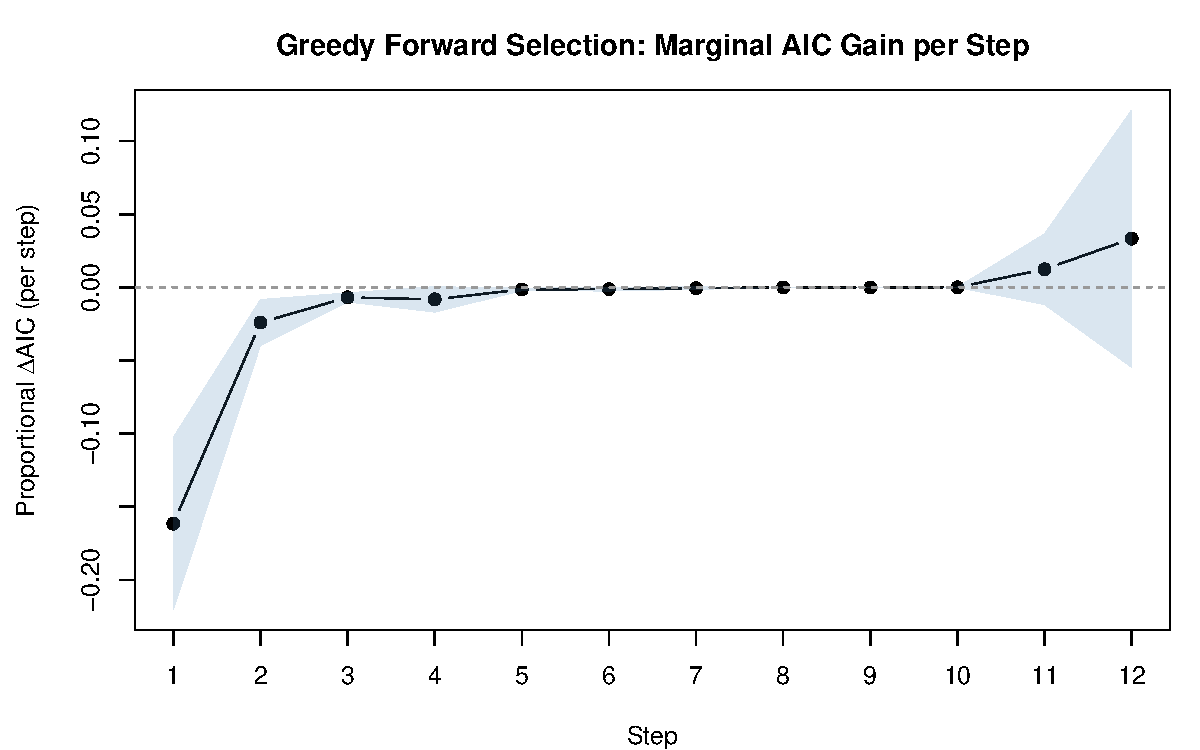
\includegraphics[width=0.85\textwidth]{greedy_aic_curve.pdf}
\caption{Domain-weighted mean per-step proportional $\Delta$AIC from greedy
forward selection ($\pm$ 95\% CI across ten domains). The marginal gain drops
sharply through step~4 and is negligible by step~5. Steps~10--12 cross into
positive territory, indicating net AIC worsening on average.}
\label{fig:elbow}
\end{figure}

\subsection{The Robust Endogenous Baseline}

Table~\ref{tab:top4freq} reports the domain-weighted frequency with which each
term appears anywhere in the first four greedy steps. This frequency-in-top-4
criterion is the primary evidence for baseline membership.

\begin{table}[H]
\centering
\caption{Domain-weighted proportion of networks selecting each term within the
first four greedy steps, overall and by ecological visibility group. The four
baseline terms (above the rule) each appear in the top-4 of over 55\% of
domains; the next candidate (OutDegSnd) appears in only 33\%.}
\label{tab:top4freq}
\begin{tabular}{lrrr}
\toprule
\textbf{Term} & \textbf{Overall} & \textbf{High-vis.} & \textbf{Low-vis.} \\
              & \textbf{(10 domains)} & \textbf{(5 domains)}  & \textbf{(5 domains)}  \\
\midrule
  SndInitiation    & 94\% & 100\% & 89\% \\
  IOviolation      & 91\% &  89\% & 92\% \\
  Repetition       & 61\% &  92\% & 30\% \\
  RecRecencyRank   & 55\% &  40\% & 70\% \\
\midrule
  OutDegSnd        & 33\% & 24\% & 42\% \\
  Imitation        & 23\% & 40\% &  5\% \\
  NOTPSnd          & 17\% & 12\% & 21\% \\
  NITPSnd          & 12\% &  2\% & 23\% \\
  WeightedRec      & 11\% &  1\% & 21\% \\
  DyadRecencyLog   &  3\% &  0\% &  7\% \\
  RRecInitiation   &  0\% &  0\% &  0\% \\
  RecRecencyLog    &  0\% &  0\% &  0\% \\
\bottomrule
\end{tabular}
\end{table}

The four-predictor model
\[
  \lambda_{ijt} = \lambda_0 \exp\!\left(
    \beta_{\text{snd}}\,A_{ijt}
    + \beta_{\text{viol}}\,V_{ijt}
    + \beta_{\text{rep}}\,R_{ijt}
    + \beta_{\text{rnk}}\,K_{ijt}
  \right)
\]
comprising \textbf{SndInitiation}, \textbf{IOviolation}, \textbf{Repetition},
and \textbf{RecRecencyRank} constitutes the robust endogenous baseline for
relational event models. SndInitiation captures whether the forward dyad has
ever fired (a binary prior-send indicator); IOviolation penalizes deviations from sequential
participation norms; Repetition adds depth to the forward-dyad signal (concentrated
prior sending); RecRecencyRank captures the recency
of the most recent reverse-dyad event ($j \to i$) via an inverse rank.
Together they characterize sequential structure and dyadic history in both
directions.

The case for including RecRecencyRank (55\%, mean selection step 4.4) rather than
the next candidate OutDegSnd (33\%, mean step 6.3) rests on the 22-percentage-point
frequency gap between them across domains. A researcher building a
general-purpose baseline could prefer the term that enters consistently early
across a wide range of contexts, but could try less-common terms in their specific domain. 

\begin{figure}[h!]
\centering
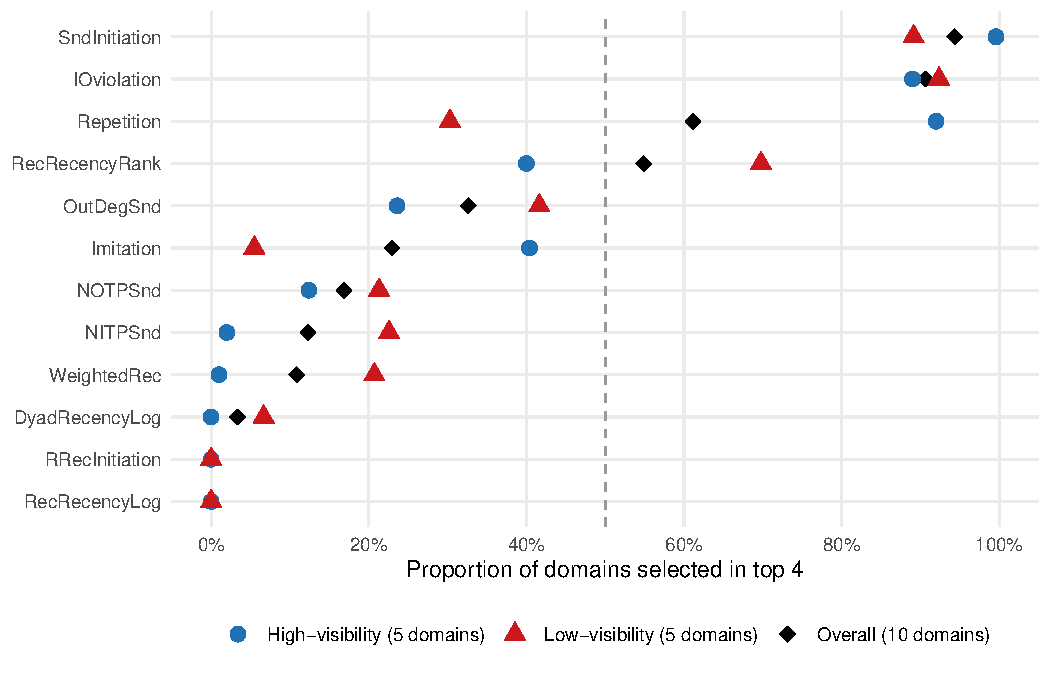
\includegraphics[width=0.88\textwidth]{freq_in_top4.pdf}
\caption{Domain-weighted proportion of domains in which each term appears
  anywhere in greedy steps~1--4 (overall and by visibility group). The four
  baseline terms (SndInitiation, IOviolation, Repetition, RecRecencyRank)
  each exceed 55\%, clearly separated from the next candidate (OutDegSnd, 33\%)
  by a 22-percentage-point gap.}
\label{fig:top4freq}
\end{figure}

Within this term set, the four-term model recovers approximately 98\% of the
domain-weighted mean proportional AIC improvement achievable at the peak of
the selection path (near step~9, $-0.204$), with wide coverage of the first four steps across all ten domains. The claim is not that these four predictors exhaust the
explanation of social interaction, nor that 97\% reflects recovery of all
possible endogenous structure --- it reflects recovery of what the twelve
specific candidate terms collectively achieve.

\subsection{Ecological Variation: High vs.\ Low Visibility}

Although the first four steps are the boundary of consistent selection in both visibility groups,
the composition of those four steps differs in ways that are theoretically
informative:

\begin{itemize}[leftmargin=2em]
  \item \textbf{SndInitiation and Repetition jointly dominate step~1 in both
        groups.} Domain-weighted, SndInitiation leads at step~1 in 63\% of
        domains overall (similar across visibility groups), with
        Repetition accounting for most of the remainder.
        Both terms capture forward-dyad history---the former as
        a binary indicator, the latter as a normalized send-share---so their
        joint dominance reflects the primacy of an actor's own prior sending
        behavior across ecological contexts.

  \item \textbf{The step-2 composition is consistent across visibility groups.}
        In both high- and low-visibility settings, \textbf{IOviolation} leads
        at step~2 (60\% high-vis, 52\% low-vis), with \textbf{RecRecencyRank}
        a close second in both groups (39\% high-vis, 34\% low-vis). Sequential
        norms and reverse-dyad recency are the primary competitors once prior
        contact is established, regardless of observational context.

  \item \textbf{SndInitiation} appears in the top~4 of 100\% of high-visibility
        domains and 89\% of low-visibility domains, and \textbf{IOviolation}
        in 89\% and 92\% respectively. Both terms are near-universal across
        visibility groups.

  \item \textbf{Repetition} shows the sharpest ecological split: 92\% in
        high-visibility domains but only 30\% in low-visibility domains.
        Repetition is the dominant step-1 term in Gang Violence and most
        single-network high-visibility domains; it is near zero in PMs, SMS,
        and Phone (Crime).

  \item \textbf{RecRecencyRank} is stronger in low-visibility settings
        (70\% low-vis vs.\ 40\% high-vis), reflecting the greater salience
        of reverse-dyad recency in conversational and messaging contexts.

  \item \textbf{Imitation} shows a high-visibility concentration
        (40\% high-vis, 5\% low-vis); once SndInitiation and Repetition
        capture forward-dyad history, imitation's marginal signal is absorbed
        in most settings but persists in some observational contexts.
\end{itemize}

Cumulative AIC recovery at step~4 is similar across visibility groups
($-0.207$ high-visibility vs.\ $-0.195$ low-visibility), indicating that
the four-term baseline captures roughly equal shares of predictable endogenous
structure in both ecological settings.


\subsection{Sensitivity Analyses}

Table~\ref{tab:aic_sensitivity} and Figure~\ref{fig:aic_sensitivity} summarize
both sensitivity criteria alongside the primary greedy frequency results.
The four baseline terms are consistently identified across all criteria.

\textbf{Univariate AIC rank (domain-weighted).}
SndInitiation (89\%) and Repetition (82\%) dominate the domain-weighted
univariate top-4, followed by Imitation (80\%) and RecRecencyRank (54\%).
IOviolation (31\%) ranks poorly on this criterion,
but the univariate criterion measures marginal fit with no other predictors
present. IOviolation's low univariate rank reflects its strong correlation with
SndInitiation and Repetition: sequential norm violations are most informative
once forward-dyad history is controlled. The univariate criterion confirms
SndInitiation and Repetition as signals, and illustrates why
path-independent marginal criteria alone are insufficient to identify the joint baseline.
Imitation's high domain-weighted univariate rank (80\%) but low greedy frequency
(23\%) is a clear illustration of path dependence: imitation is a strong
univariate predictor whose signal is absorbed once SndInitiation and Repetition
enter the model.

\textbf{Take-one-out from the full 12-term model (TOO-12).}
For each network, all twelve terms are ranked by their AIC increase when
dropped from the full joint model; a term is flagged if it ranks in the
top four (i.e., is among the four most costly to remove). This criterion
is directly parallel to the other two columns: all three report the
domain-weighted proportion of networks where each term ranks in the top four
on the relevant criterion, and none pools heterogeneous AIC magnitudes across
sequences of different lengths.

SndInitiation and IOviolation each rank in the top-4 by TOO-12 in 95\% of
domains, confirming both are indispensable in the joint model despite
IOviolation's modest univariate rank. Repetition (58\%) and RecRecencyRank
(57\%) are the next most consistently costly to drop, clearly above all
non-baseline terms. OutDegSnd (39\%) has a higher TOO-12 top-4 rate than its
greedy frequency (33\%), reflecting its genuine joint-model contribution even
when it does not enter early in the greedy path.

Imitation's TOO-12 top-4 rate collapses to 3\%---despite its 80\% univariate
rank---confirming that its signal is almost entirely absorbed by SndInitiation
and Repetition in the joint model. DyadRecencyLog, RRecInitiation, and
RecRecencyLog each score 0\% on all three criteria.

\begin{table}[H]
\centering
\small
\caption{Three sensitivity criteria for the robust endogenous baseline, each
reported as the domain-weighted proportion of networks where the term ranks
in the top four on the relevant criterion. \textit{Greedy top-4}: top-four
greedy selection steps (main analysis, $N=217$). \textit{Univariate top-4}:
top-four by step-1 univariate AIC rank (path-independent). \textit{TOO-12
top-4}: top-four by AIC increase when dropped from the full 12-term joint
model (most costly to remove).}
\label{tab:aic_sensitivity}
\begin{tabular}{lccc}
\toprule
\textbf{Term} & \textbf{Greedy top-4} & \textbf{Univ.\ top-4} & \textbf{TOO-12 top-4} \\
\midrule
  SndInitiation  & 94\% & 89\% & 95\% \\
  IOviolation    & 91\% & 31\% & 95\% \\
  Repetition     & 61\% & 82\% & 58\% \\
  RecRecencyRank & 55\% & 54\% & 57\% \\
\midrule
  OutDegSnd      & 33\% &  2\% & 39\% \\
  Imitation      & 23\% & 80\% &  3\% \\
  NOTPSnd        & 17\% & 15\% & 23\% \\
  NITPSnd        & 12\% &  1\% &  2\% \\
  WeightedRec    & 11\% & 47\% & 29\% \\
  DyadRecencyLog &  3\% &  0\% &  0\% \\
  RRecInitiation &  0\% &  0\% &  0\% \\
  RecRecencyLog  &  0\% &  0\% &  0\% \\
\bottomrule
\end{tabular}
\end{table}



% -------------------------------------------------------
\section{Discussion}

\paragraph{A robust floor, not a sufficient ceiling.}
The wide coverage of the first four steps --- each baseline term appearing in
the top four of 55--94\% of domains --- and the clear separation in
domain-weighted frequency-in-top-4 between the four baseline terms and the
next candidate OutDegSnd (33\%), supports the claim that these four terms
constitute a robust endogenous baseline.
The claim is emphatically not that they are sufficient. Social interaction is
shaped by institutional context, status and demographic characteristics, spatial
and organizational structure, and much else. The four-term model is best
understood as the endogenous foundation that any well-specified REM should
include before introducing substantive theoretical covariates. Failure to do so
risks conflating structural inertia---actors returning to established partners,
honoring sequential obligations---with the effects of the exogenous variables
under study.

\paragraph{Imitation and triadic closure as non-universal terms.}
Imitation and repetition are conceptually distinct: imitation requires that
others' targeting behavior be observable, while repetition reflects a dyadic
inertia that operates regardless of ecological context. Domain-weighted across
all ten domains, imitation does not enter reliably within the top four steps
(23\% overall), and its TOO-12 top-4 rate collapses to 3\% in the joint model.
The triadic closure terms (NOTPSnd, NITPSnd) follow the same pattern: both score
near zero on greedy frequency and TOO-12. In each case, the mechanism is real
but redundant conditional on forward-dyad history: once SndInitiation and
Repetition establish who has sent to whom, the additional signal from others'
behavior or shared third parties is largely absorbed.

Imitation's weak overall showing, however, masks a meaningful ecological split.
In high-visibility settings --- classrooms, public conflict, broadcast contexts
where others' targeting behavior is observable --- imitation appears in the top
four of 40\% of domains, compared to only 5\% in low-visibility settings.
Researchers working in high-visibility contexts should treat imitation as a
strong candidate for inclusion beyond the four-term baseline, not merely an
optional theoretical term. In low-visibility settings, imitation can safely be
omitted. Triadic closure terms show no comparable ecological recovery and remain
weak candidates across all settings.

\paragraph{Domain patterns: conflictual versus affiliative interaction.}
An ecological pattern visible in the valence-split heatmap concerns
the composition of step-2 selection between conflictual and affiliative contexts.
In conflictual domains (gang violence, international conflict), IOviolation and
RecRecencyRank are nearly tied at step~2 (50\% and 48\% respectively). In
affiliative domains, IOviolation leads step~2 (57\%), with RecRecencyRank
accounting for most of the remainder (34\%).

Both patterns are consistent with distinct behavioral logics. In adversarial
contexts, the recency of being targeted is a strong competitor to sequential
norms: retaliatory dynamics produce a reverse-dyad recency signal, and an actor
who was recently struck is more likely to respond. In affiliative settings,
sequential participation norms take clear precedence---conversation partners
alternate turns. The four-term baseline holds across both valence groups, but the relative weight of
sequential ordering versus reverse-dyad recency varies with context.

\paragraph{Redundant reciprocity terms: nothing to add over and above RecRecencyRank.}
Three terms --- RecRecencyLog, RRecInitiation, and DyadRecencyLog --- score
zero on greedy frequency and TOO-12 across the full corpus. All three are
reciprocity-adjacent: RecRecencyLog is the clock-time analog of RecRecencyRank;
RRecInitiation is the binary indicator of whether $j$ has ever sent to $i$; and
DyadRecencyLog captures elapsed time since $i$ last sent to $j$. Their
consistent failure to enter the top four reflects not irrelevance but
redundancy --- once RecRecencyRank, SndInitiation, and Repetition are in the
model, these terms add nothing that is not already captured. RecRecencyLog is
the clearest case: its rank-based analog, RecRecencyRank, enters the top-4 of
55\% of domains (domain-weighted mean selection step 4.4), while RecRecencyLog
is not selected within the first four steps in any network (mean selection step
10.5). The displacement of the clock-time measure by its rank analog is not an
artifact of step order: as a standalone first-selected term, RecRecencyRank
dominates RecRecencyLog across networks, indicating that the \emph{ordinal
position} of a reverse-dyad event carries more predictive information than
logged elapsed time.

\paragraph{SndInitiation and the case for separable estimation.}
The consistent early selection of SndInitiation---whether sender $i$ has ever
previously contacted receiver $j$---at step~1 in 63\% of domains (domain-weighted)
carries a structural implication beyond its role as a baseline term.
SndInitiation is a binary absorbing state: once $i$ has ever sent to $j$, the
indicator permanently equals one for all subsequent $i \to j$ events. This
partitions the event sequence into two qualitatively distinct regimes:
\emph{initiation events}, in which $i$ contacts $j$ for the first time, and
\emph{continuation events}, in which $i$ returns to an already-contacted $j$.
A pooled REM averages these two regimes with a single parameter set, but the
mechanisms governing them may differ in direction or magnitude. The consistent early selection of SndInitiation indicates
that the prior-send binary is a fundamental partition of the risk set across
interaction settings, and motivates \emph{separable} relational event models
that assign distinct parameter vectors to initiation and continuation events.
Full development of separable REMs is left for subsequent work.

\paragraph{Correlation structure and selection stability.}
Several terms in the twelve-term set share variance in ways that affect greedy
selection order within steps~2--4. Repetition and OutDegSnd both depend on $i$'s
prior sending history but in complementary directions: Repetition rewards
concentration on one partner while OutDegSnd rewards breadth. RecRecencyRank and RecRecencyLog both capture reverse-dyad recency ($j \to i$);
the consistent displacement of the log-time measure is discussed above.
SndInitiation and Repetition are correlated, both capturing forward-dyad history
at different granularities. The relationship between IOviolation and SndInitiation is also worth noting.
IOviolation's low univariate rank (31\%) but high TOO-12 rate (95\%) marks it
as a conditionally important term: its sequential-ordering signal is most
distinctively informative once the dyadic baseline established by SndInitiation
and Repetition is already in the model. Again, this conditional dependence also has implications
for separable estimation: a separable REM would use SndInitiation as the
partition criterion, splitting the risk set into initiation events (first contact
on a dyad) and continuation events (returns to an established dyad). IOviolation
may carry far more weight in the continuation sub-model, where
established interaction patterns make sequential norm violations more
diagnostically meaningful, though it is not logically restricted to that
sub-model. The joint-model results reported here pool both regimes; separable
estimation would clarify the extent to which IOviolation's contribution is
concentrated in continuation events.


The sensitivity analyses help distinguish three types of terms.
\textit{Consistent terms} (SndInitiation, Repetition) are strong on every
criterion: high greedy frequency, high univariate rank, and high TOO-12 top-4 rate.
\textit{Conditionally important terms} (IOviolation) are weak univariately but
indispensable in the joint model: IOviolation's TOO-12 top-4 rate (95\%) matches
SndInitiation's exactly, confirming it is among the costliest terms to remove
despite its 31\% univariate rank.
\textit{Path-dependent terms} (Imitation, WeightedRec) have high univariate ranks
but low greedy frequencies and near-zero TOO-12 top-4 rates, confirming their
signal is absorbed by forward-dyad history terms once those enter the model.
The four-term baseline is robust to all three types: none of the non-baseline
terms displaces a baseline term on any criterion.

\paragraph{A note on the self-generating structure of interaction.}
The dominance of a small set of dyadic event-history statistics across ten
structurally diverse settings raises a broader question: how much of observed
interaction structure is self-generated by prior interaction, rather than imposed
by actors' social positions? The present study cannot answer that question ---
we include no exogenous covariates, so we cannot partition explained variance
between endogenous and exogenous sources. What the findings do show is that
a compact set of event-history terms competes well for AIC improvement within
this candidate set across structurally diverse domains, which is consistent with
the hypothesis that much of what looks like structure may itself be a residue of
prior event history. More broadly, the cross-domain
stability of a four-term core covering dyadic contact, sequential obligation,
and reverse-dyad recency --- holding from private messaging to gang violence ---
is consistent with the hypothesis that a small number of behavioral mechanisms
may constitute universal building blocks of directed social interaction, operating
beneath the surface of contextual variation. Whether that universality is rooted
in cognitive constraints, strategic logic, or evolved coordination tendencies
remains an open question. Distinguishing genuine endogenous habituation from
stable exogenous confounds, and testing the universality claim against a broader
range of interaction types, are natural targets for future work.

% -------------------------------------------------------
\section{Limitations}

Three limitations bear on generalization. First, the
proportional $\Delta$AIC is bounded above by the twelve-term candidate set: the
97\% figure reflects recovery of what these twelve terms collectively achieve,
not 97\% of all predictable endogenous structure. Terms not represented include
receiver-side recency (log time since $j$ last received from anyone), sender
indegree (how frequently $i$ has been targeted by others), decomposed
participation shifts (the three shift types composing IOviolation treated
separately), and higher-order closure paths. The core finding is robust to
the present term set, though further terms not evaluated here could in principle
alter the specific composition of the baseline.

Second, greedy forward selection is path-dependent: a term that loses the
step-1 competition is subsequently evaluated with its variance partly absorbed
by earlier entrants. Two sensitivity analyses address this concern. Domain-weighted
univariate AIC rank at step~1 is entirely path-free and confirms SndInitiation and
Repetition as strong marginal predictors. Take-one-out from the full 12-term
model confirms that all four baseline terms are indispensable in the joint
context (minimum TOO-12 top-4 rate: RecRecencyRank 57\%; IOviolation: 95\%)
despite IOviolation's modest univariate rank. Together these criteria
bracket the greedy result from two directions---marginal importance and full
joint importance---consistently supporting the four-term baseline. The precise
ordering of entry within steps~2--4 remains sensitive to collinearity and should
not be read as a strict priority ranking; the frequency-in-top-4 separation is
the robust claim.

Third, the high/low visibility categorization is treated as a categorical
variable. The underlying construct---observational accessibility of others'
interaction histories---likely varies continuously across settings and may be
partially mis-specified for borderline domains such as glance networks.


% -------------------------------------------------------
\section{Conclusion}

Four terms --- SndInitiation, IOviolation, Repetition, and RecRecencyRank ---
appear in the greedy top-four selection path of 55--94\% of domain proportions
across ten social domains (domain-weighted), with a 22-percentage-point gap to
the next candidate (OutDegSnd, 33\%) and wide coverage across the first four steps.
Together they recover approximately 97\% of the maximum AIC improvement
achievable within this twelve-term candidate set (domain-weighted peak:
$-0.204$ at step~9). Two path-independent sensitivity analyses corroborate
the greedy result: domain-weighted univariate AIC rank confirms SndInitiation
and Repetition as the dominant pure signals; take-one-out from the full 12-term
model confirms that all four terms are indispensable in the joint fit, with
SndInitiation and IOviolation each ranking in the top-4 costliest to drop in 95\% of networks.

These four terms represent three behavioral mechanisms --- sequential ordering,
dyadic persistence, and reverse-dyad recency --- that operate across ecological
contexts from private messaging to gang violence. They are not a sufficient model,
but they are a consistent floor. Notably, imitation and triadic closure ---
terms that have attracted considerable attention in the network literature ---
do not belong in this floor: their signal is absorbed by forward-dyad history
and they add little in a joint specification. Include the four baseline terms
before domain-specific covariates, and the risk of misattributing structural
inertia to exogenous variables is substantially reduced.

% -------------------------------------------------------
\bibliography{cites}
\bibliographystyle{ajs}

% -------------------------------------------------------
\appendix

\section{Data Sources}
\label{sec:datasources}

The 217 sequences span ten social domains drawn from eight empirical corpora and two sets of synthetic networks. Each domain is assigned to a high- or low-visibility group based on whether participants can observe each other's interaction histories during the interaction.

\paragraph{Classroom interactions (high-visibility, $n = 5$).}
Classroom interaction sequences from McFarland's study of high-school classroom dynamics \citep{mcfarland_classroom}, distributed via the \texttt{networkDynamicData} R package \citep{bender2016package}. Each sequence records directed talk events among students and teachers in a single class session (mean: 691 events; 21 participants). Classroom interaction is high-visibility: participants are co-present and can observe who is addressing whom.

\paragraph{Email (low-visibility, $n = 33$).}
Email sequences drawn from the SNAP email-Eu-core-temporal dataset \citep{snapnets}, comprising internal email among members of a European research institution. Each sequence is a 5,001-event window drawn from a single department's communication record. Sender-recipient pairs are not publicly observable, placing email in the low-visibility group.

\paragraph{Gang violence (high-visibility, $n = 100$).}
Synthetic directed networks calibrated to empirical gang conflict data from Los Angeles \citep{tita2011spatializing,gravel2023rivalries}. Each network consists of 450 directed violent events among 33 actor-gangs. Gang violence is high-visibility: retaliatory conflicts are publicly known within the gang ecology.

\paragraph{Glance networks (low-visibility, $n = 62$).}
Face-to-face gaze sequences from a laboratory study of small group interaction, distributed via \texttt{networkDynamicData} \citep{bender2016package}. Each sequence is a 10,000-event window; groups range from 5 to 8 participants. Despite the face-to-face setting, individual gaze is not publicly broadcast within the group, placing glance networks in the low-visibility group (borderline case).

\paragraph{Private messages (low-visibility, $n = 8$).}
Private message sequences from the UCI online community messaging dataset \citep{panzarasa2009patterns}. Each sequence is a 7,001-event window drawn from a single cohort of university students. Private messages are not observable to third parties.

\paragraph{Phone calls --- DoD (high-visibility, $n = 1$).}
A single directed phone-call sequence from a Department of Defense military exercise (TSOF dataset), recording 196 calls among 94 participants. Communication in a coordinated military exercise is treated as high-visibility because participants share a command structure with observable communication patterns.

\paragraph{SMS (low-visibility, $n = 3$).}
Mobile SMS sequences drawn from SNAP \citep{snapnets}, each a 5,001-event window from a large mobile communication dataset. SMS is low-visibility: messages are private.

\paragraph{Twitter / EMO (high-visibility, $n = 9$).}
Twitter interaction sequences from the EMO corpus \citep{renshaw2023modeling}, recording directed mentions and replies during a crisis communication exercise. Each sequence records 227 events among 20 users. Twitter interaction is public and high-visibility.

\paragraph{International conflict (high-visibility, $n = 1$).}
A single directed interaction sequence constructed from the Interstate War Battle (IWB) dataset \citep{miniwd}, recording 1,708 militarized actions among 95 state actors across multiple interstate conflicts (1823--2003). Interstate conflict is high-visibility: military operations are observable by adversaries and third parties.

\paragraph{Phone calls --- organized crime (low-visibility, $n = 1$).}
A single directed phone-call sequence from a wiretapped organized crime network. Phone calls between criminal actors are private and low-visibility by design.

\medskip
\noindent The analysis uses domain-weighted averages throughout: each domain contributes equally regardless of how many sequences it contributes to the corpus (the two largest domains, Gang Violence with $n=100$ and Glances with $n=62$, would otherwise account for 75\% of the 217 sequences).

\section{Coefficients from Network-Specific Final Models}

Table~\ref{tab:final_coefs} reports the mean coefficient and mean
model-estimated standard error across the 216 networks for which
final greedy models were successfully fit (217 total minus 1
network that did not converge).
Each network's ``final model'' is the model at the last greedy step
where proportional $\Delta\text{AIC}$ was still negative; the number of
terms included therefore varies by network (steps 5--12, mean $\approx 7.6$).
Because $N$ varies by row, the mean SE summarises typical within-model
precision for that term rather than variability across networks.
Stars reflect the ratio mean~coef / mean~SE and indicate that the average
estimate is large relative to its average uncertainty across the networks
that selected it.

\begin{table}[htbp]
\centering
\small
\caption{Mean coefficient and mean model SE (in parentheses) across network-specific final greedy models, by visibility group ($n=216$; one network excluded due to non-convergence). $N$ is the number of networks whose final model included each term. Stars indicate mean~coef / mean~SE $\geq 1.96$ ($^*$), $2.58$ ($^{**}$), or $3.29$ ($^{***}$), reflecting average within-model precision. Terms with $N \leq 3$ appear in very few networks; their entries are included for completeness but should not be treated as evidence of cross-network generalizability.}
\label{tab:final_coefs}
\begin{tabular}{lcrcrr}
\toprule
& \multicolumn{2}{c}{High-vis} & \multicolumn{2}{c}{Low-vis} & Overall ($n=216$) \\
\cmidrule(lr){2-3}\cmidrule(lr){4-5}
Term & Mean (SE) & $N$ & Mean (SE) & $N$ & Mean (SE) \\
\midrule
\multicolumn{6}{l}{\textit{Forward-dyad history}} \\
\quad SndInitiation & 1.192 (0.188)*** & 103 & 2.543 (0.128)*** & 103 & 1.867 (0.158)*** \\
\quad Repetition & 1.289 (0.292)*** & 103 & 2.952 (0.084)*** & 103 & 2.120 (0.188)*** \\
\multicolumn{6}{l}{\textit{Reverse-dyad history}} \\
\quad RecRecencyRank & 1.603 (0.148)*** & 103 & 1.239 (0.050)*** & 92 & 1.431 (0.102)*** \\
\quad RecRecencyLog & -0.056 (0.088) & 2 & -0.530 (0.010)*** & 1 & -0.214 (0.062)*** \\
\quad RRecInitiation & 0.256 (0.416) & 2 & -0.400 (0.070)*** & 1 & 0.037 (0.301) \\
\quad WeightedRec & -0.073 (0.210) & 41 & -0.181 (0.055)** & 93 & -0.148 (0.102) \\
\multicolumn{6}{l}{\textit{Popularity, sender activity, triadic}} \\
\quad Imitation & 0.237 (0.222) & 38 & -0.084 (0.056) & 84 & 0.016 (0.107) \\
\quad OutDegSnd & 1.409 (0.222)*** & 88 & 1.564 (0.076)*** & 80 & 1.483 (0.153)*** \\
\quad DyadRecency & -0.343 (0.089)*** & 2 & -0.104 (0.010)*** & 1 & -0.263 (0.062)*** \\
\quad NOTPSnd & 0.667 (0.132)*** & 100 & 0.676 (0.100)*** & 95 & 0.672 (0.117)*** \\
\quad NITPSnd & 0.495 (0.144)*** & 60 & 0.128 (0.097) & 79 & 0.287 (0.117)* \\
\multicolumn{6}{l}{\textit{Sequential ordering}} \\
\quad IOviolation & -0.593 (0.145)*** & 101 & -0.389 (0.041)*** & 105 & -0.489 (0.092)*** \\
\bottomrule
\end{tabular}
\end{table}


\end{document}
